\chapter{Results and Analysis}
\label{chap5}

To perform the tests described in \autoref{tab:instr_skip_test} we follow the steps described in \autoref{subsec:sim_glitch}.

\section{PPA comparison}
\label{sec:synth_comparison}

Results of synthesis of both cores as well as number of cycles needed to complete the test program in \autoref{app:helloworldC} is shown in \autoref{tab:ppa_results}. The relative difference from the single core to dual-cores is shown in the table.

\begin{table}[h]
\centering
\caption{PPA results from simulation and synthesis of both setups.}
\label{tab:ppa_results}
\begin{tabular}{c|ccc}
\toprule 
Setup & Area[$pm^2$] & Power[$\mu W$] & Clock Cycles\\
\midrule
\rowcolor{black!20} CV32E40S & 63121.093 & 113.007 & 18424\\
CV32E40S Dual-Core & 65214.732[$+3.3\%$] & 144.482[$+27.9\%$] & 17446[$-5.3\%$] \\
\bottomrule
\end{tabular}
\end{table}

\section{Instruction Skipping}
\label{sec:instr_skip_result}

\subsection{CV32E40S}
\label{subsec:single_instr_skip}

\subsubsection{Skipping function call}

 From the log file, we can see that the \textit{c.jal} instruction is logged at 1752ns. To skip this instruction the program counter needs to be skipped in the \textit{IF} stage, which is 3 cycles before \textit{WB}. The system clock has a period of 3ns, meaning the glitch is injected at 1743ns. The \textit{c.jal} is located at the address: \textit{0x0000044c}. Forcing the program counter to the next address \textit{0x0000044e} for a duration of 3ns will simulate an instruction skip. The address of the next instruction is only 2 away because the \textit{jal} is a 16-bit compressed instruction.

Glitching of the core was done successfully. The waveforms from simulation are shown in \autoref{fig:instr_skip_single_wave}. From the figure one can see that the glitch is detected immediately. 

\begin{figure}[h!]
    \centering
    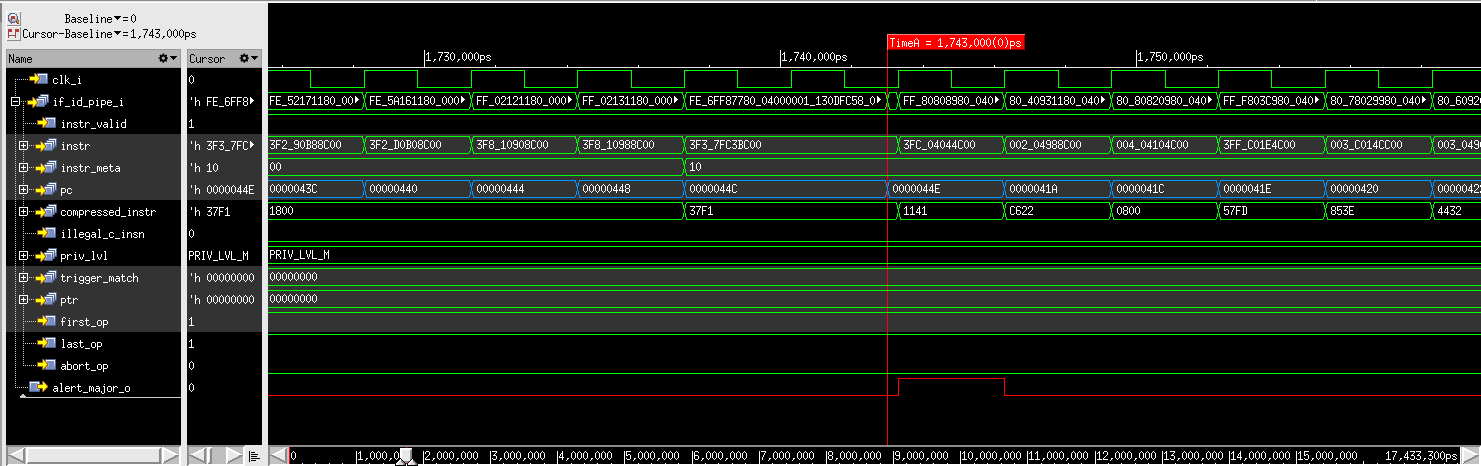
\includegraphics[width=\textwidth]{docs/images/instr_skip_glitch_injection_single_core.png}
    \caption{Waveforms from simulated instruction skip on CV32E40S.}
    \label{fig:instr_skip_single_wave}
\end{figure}

\subsubsection{Skipping out of while loop}

From the log file, we can see that the \textit{c.j} instruction is called 10 times. We skip the one logged at 1833ns. To skip this instruction the program counter needs to be skipped in the \textit{IF} stage, which is 3 cycles before the \textit{WB}. The \textit{c.j} is located at \textit{0x0000047a}. Forcing the program counter to the next address \textit{0x0000047c} for a duration of 3ns will simulate an instruction skip. This address is only 2 away because the \textit{j} is a 16-bit compressed instruction. 

Glitching out of the while loop was not successful. This is possibly due to other branch instructions from the loop that are also inside the pipeline. The attempted instruction skip is still detected and a major alert is raised. This can be seen in the simulation waveforms in \autoref{fig:instr_skip_loop_single_wave}. 

\begin{figure}[h!]
    \centering
    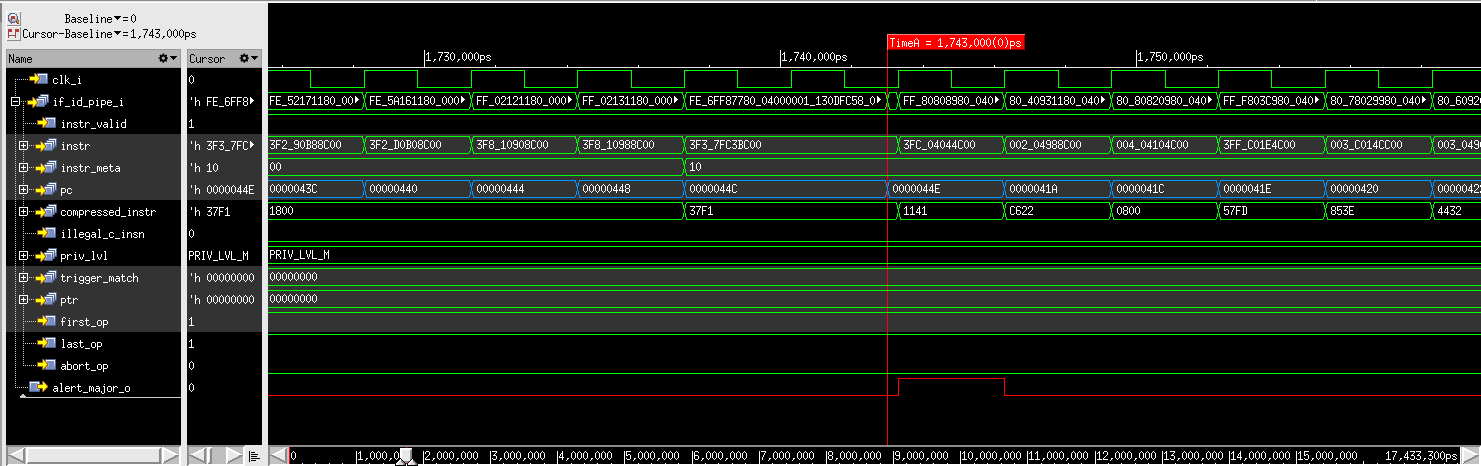
\includegraphics[width=\textwidth]{docs/images/instr_skip_glitch_injection_single_core.png}
    \caption{Waveforms from simulated instruction skip on CV32E40S.}
    \label{fig:instr_skip_loop_single_wave}
\end{figure}

\subsubsection{Skipping directly to end}

As mentioned earlier, an attacker can potentially glitch directly to the end of the program if they have some way of manipulating the code in the boot-loader. To simulate this, the program counter is forced to the address of the instruction after the while loop, \textit{0x00000482}. This force happens as soon as the main program is entered, which is at 1737ns.

This glitch attack was not successful. However, no major alert was raised by the core as can be seen in \autoref{fig:direct_skip_single_wave}. This glitch therefore bypassed the PCH feature. 

\begin{figure}[h!]
    \centering
    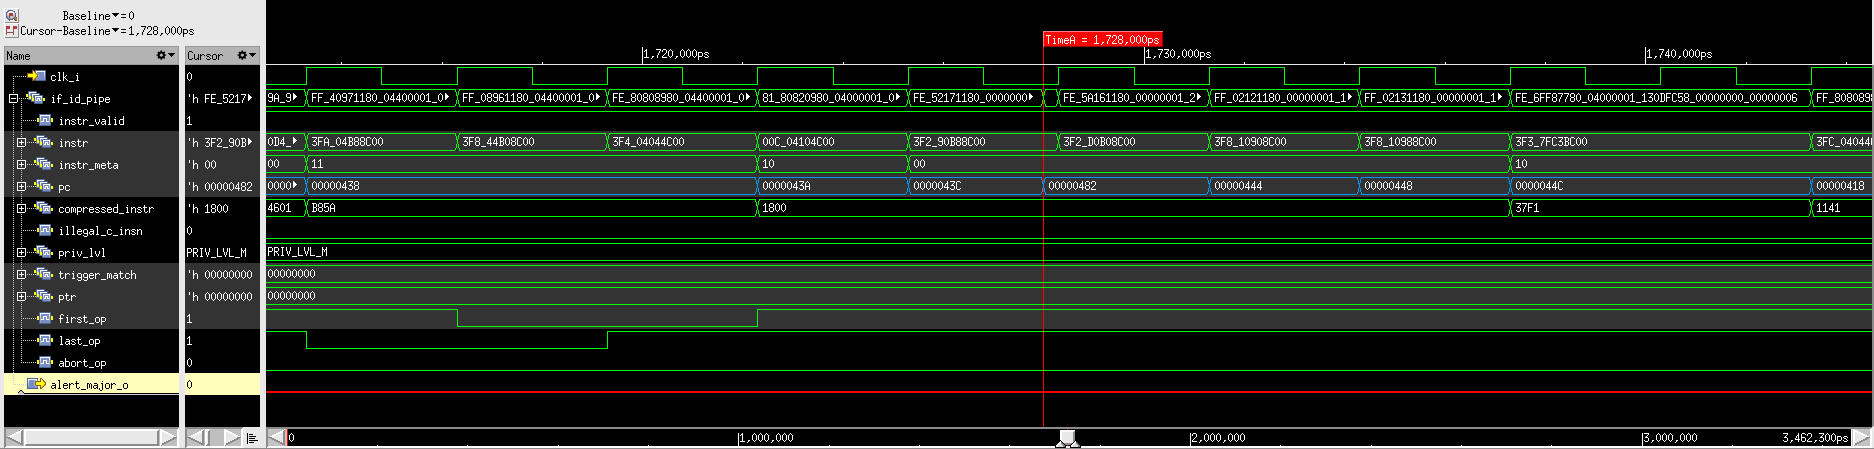
\includegraphics[width=\textwidth]{docs/images/direct_skip_single_core.png}
    \caption{Waveforms from simulated direct instruction skip on CV32E40S.}
    \label{fig:direct_skip_single_wave}
\end{figure}

\subsection{Dual-Core Lockstep}
\label{subsec:dual_instr_skip}

\subsubsection{Skipping function call}

The call to the \textit{c.jal} instruction occurs at 1731ns. The program counter is glitched to the address \textit{0x0000044e}. 

\begin{figure}[h!]
    \centering
    \includegraphics[width=\textwidth]{docs/images/instr_sk.png}
    \caption{Waveforms from simulated direct instruction skip on CV32E40S.}
    \label{fig:direct_skip_single_wave}
\end{figure}


\subsubsection{Skipping out of while loop}

The call to the \textit{c.j} instruction occurs first at 1809ns. The program counter is glitched to the address \textit{0x0000047c}.

\subsubsection{Skipping directly to end}

The call to the \textit{main} function occurs at 1710ns. The program counter is glitche dto the address \textit{0x00000482}.


\section{Coverage Test}
\label{sec:cov_test_result}



\textbf{Instruction to be glitched:}
\begin{lstlisting}
       30003.000 ns | 0000672c | memchr syscalls.c 379 - beq x14,x10,66b4 <memchr+0x3c>
\end{lstlisting}

In order to glitch the loop we need to make the program skip the instruction that happens at 29991.000 ns. This is a bne instruction that keeps us in the loop. Next instruction occurs at 29997 and we must therefore chang ethe program counter before this. 

Glitch 6734 to 673c

Count lagret i x8 
Verdien 10 lagret i x9

\section{Layout comparisons}

\subsection{Can this be implemented in read hardware?}
\begin{itemize}
    \item Compare performance 
    \item Compare area
    \item Compare Timing 
    \item Compare simulated power usage
    \item Compare glitch detection
\end{itemize}

\section{Why is this solution good/bad}

Synthesis results no pc hardening and dual core:

Area: 65214.732
Power: 1.44482mW
